% !TEX encoding = UTF-8
% !TEX TS-program = pdflatex
% !TEX root = ../tesi.tex

%**************************************************************
\chapter{Analisi dei requisiti}
\label{cap:descrizione-stage}
%**************************************************************
In questa sezione vengono illustrati i requisiti individuati per il progetto SyncRec.

\section{Tipologie di utenti}
Questa sezione ha lo scopo di dettagliare gli attori individuati; ciascun attore si differenzia dagli altri per i permessi di accesso a determinate parti del sistema:
\begin{itemize}	
	\item \textbf{\nonlogged:} utente che non ha eseguito il \textit{login} presso l'applicazione, nel corso del lavoro svolto dal laureando non sono stati modellati casi d'uso per questo attore.
	\item \textbf{\loggedusr:} utente che ha effettuato l'accesso alla piattaforma SyncRec;
	\item \textbf{\applicant:} utente a cui è stato inviato un link specifico per la compilazione dello skillmatrix prima dello svolgimento di un colloquio lavorativo. 
\end{itemize}

\section{Casi d'uso}
La sezione presenta i casi d'uso individuati per l'intero progetto SyncRec.

%\subsection{UC-}
%\begin{itemize}
%\item \textbf{Attori:}
%\item \textbf{Precondizione:}
%\item \textbf{Scenario Principale:}
%\begin{enumerate}
%	\item 
%\end{enumerate}
%\item \textbf{PostCondizione:}
%\item \textbf{Estensioni:}
%\end{itemize}
\vspace{0.5em}
\begin{figure}[!h] 
	\centering 
	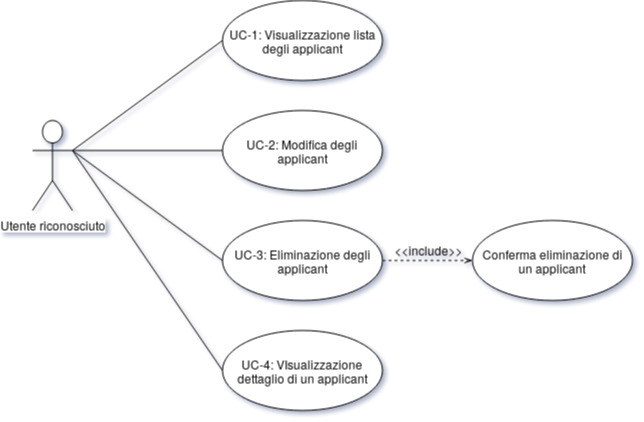
\includegraphics[width=1\columnwidth]{immagini/usecase/UC1} 
	\caption{Diagramma di Use Case da 1 a 4}
	\label{figura:uc-1}
\end{figure}


\subsection{UC-1: Visualizzazione lista degli\applicant}
\begin{itemize}
	\item \textbf{Attori:}\loggedusr
	\item \textbf{Precondizione:} l'utente si trova nella vista di visualizzazione lista degli applicant.
	\item \textbf{Scenario Principale:} 
		\begin{enumerate}
			\item l'utente visualizza il cognome dell'applicant; 
			\item l'utente visualizza il nome dell'applicant;
			\item l'utente visualizza l'email dell'applicant;
		\end{enumerate}
	\item \textbf{PostCondizione:} l'utente si trova nella vista di visualizzazione lista degli applicant.
\end{itemize}

\subsubsection{\underline{UC-1.1: Visualizzazione dettaglio di un\applicant}}
\begin{itemize}
	\item \textbf{Attori:}\loggedusr
	\item \textbf{Precondizione:} l'utente si trova nella vista di visualizzazione lista degli applicant. 
	\item \textbf{Scenario Principale:}
	\begin{enumerate}
		\item l'utente clicca sul pulsante relativo a un applicant;
		\item l'utente viene reindirizzato alla vista di dettaglio di un applicant;
		\item l'utente visualizza tramite la vista il dettaglio degli applicant.
	\end{enumerate}
	\item \textbf{PostCondizione:} l'utente si trova nella vista di dettaglio di un applicant;
\end{itemize}


\subsection{UC-2: Modifica di un \applicant}
\begin{itemize}
	\item \textbf{Attori:} Utente riconosciuto
	\item \textbf{Precondizione:}  l'utente si trova nella vista di dettaglio di un applicant;
	\item \textbf{Scenario Principale:}
	\begin{enumerate}
		\item l'utente clicca sul campo dati di un applicant che desidera modificare;
		\item l'utente visualizza il  widget di modifica per il campo dati
		relativo;
		\item l'utente inserisce le modifiche desiderate.
	\end{enumerate}
	\item \textbf{PostCondizione:} 
	\begin{enumerate}
		\item l'utente visualizza il campo dati modificato;
		\item l'utente si trova nella vista di dettaglio di un applicant.
	\end{enumerate}
	
\end{itemize}

\begin{figure}[!h] 
	\centering 
	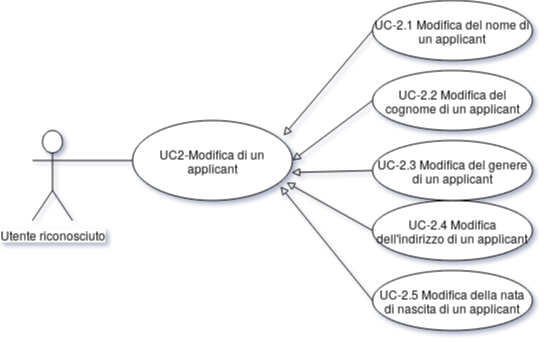
\includegraphics[width=1\columnwidth]{immagini/usecase/UC3} 
	\caption{Diagramma sottocasi UC-2}
	\label{figura:uc-3}
\end{figure}


\subsubsection{\underline{UC-2.1: Modifica del nome di un \applicant}}
\begin{itemize}
	\item \textbf{Attori:} Utente riconosciuto
	\item \textbf{Precondizione:}  l'utente si trova nella vista di dettaglio di un applicant;
	\item \textbf{Scenario Principale:}
	\begin{enumerate}
		\item l'utente clicca sul box di testo relativo al nome;
		\item l'utente visualizza il  widget di inserimento testo relativo al nome;
		\item l'utente inserisce le modifiche desiderate.
	\end{enumerate}
	\item \textbf{PostCondizione:} 
	\begin{enumerate}
		\item l'utente visualizza il campo dati modificato;
		\item l'utente si trova nella vista di dettaglio di un applicant.
	\end{enumerate}
	
\end{itemize}

\subsubsection{\underline{UC-2.2: Modifica del cognome di un \applicant}}
\begin{itemize}
	\item \textbf{Attori:} Utente riconosciuto
	\item \textbf{Precondizione:}  l'utente si trova nella vista di dettaglio di un applicant;
	\item \textbf{Scenario Principale:}
	\begin{enumerate}
		\item l'utente clicca sul box di testo relativo al cognome;
		\item l'utente visualizza il  widget di inserimento testo relativo al cognome;
		\item l'utente inserisce le modifiche desiderate.
	\end{enumerate}
	\item \textbf{PostCondizione:} 
	\begin{enumerate}
		\item l'utente visualizza il campo dati modificato;
		\item l'utente si trova nella vista di dettaglio di un applicant.
	\end{enumerate}
	
\end{itemize}

\subsubsection{\underline{UC-2.3: Modifica del genere di un \applicant}}
\begin{itemize}
	\item \textbf{Attori:} Utente riconosciuto
	\item \textbf{Precondizione:}  l'utente si trova nella vista di dettaglio di un applicant;
	\item \textbf{Scenario Principale:}
	\begin{enumerate}
		\item l'utente clicca sul box di testo relativo al nome;
		\item l'utente visualizza il  menù a tendina relativo al genere;
		\item l'utente seleziona il dato dal menù a tendina.
	\end{enumerate}
	\item \textbf{PostCondizione:} 
	\begin{enumerate}
		\item l'utente visualizza il campo dati modificato;
		\item l'utente si trova nella vista di dettaglio di un applicant.
	\end{enumerate}
	
\end{itemize}

\subsubsection{\underline{UC-2.4: Modifica dell'indirizzo di un \applicant}}
\begin{itemize}
	\item \textbf{Attori:} Utente riconosciuto
	\item \textbf{Precondizione:}  l'utente si trova nella vista di dettaglio di un applicant;
	\item \textbf{Scenario Principale:}
	\begin{enumerate}
		\item l'utente clicca sul box di testo relativo all'indirizzo;
		\item l'utente visualizza il  widget di inserimento testo relativo all'indirizzo;
		\item l'utente inserisce le modifiche desiderate.
	\end{enumerate}
	\item \textbf{PostCondizione:} 
	\begin{enumerate}
		\item l'utente visualizza il campo dati modificato;
		\item l'utente si trova nella vista di dettaglio di un applicant.
	\end{enumerate}
	
\end{itemize}

\subsubsection{\underline{UC-2.5: Modifica della data di nascita di un \applicant}}
\begin{itemize}
	\item \textbf{Attori:} Utente riconosciuto
	\item \textbf{Precondizione:}  l'utente si trova nella vista di dettaglio di un applicant;
	\item \textbf{Scenario Principale:}
	\begin{enumerate}
		\item l'utente clicca sul box di testo relativo alla data di nascita;
		\item l'utente visualizza il  widget di inserimento data relativo alla data di nascita;
		\item l'utente inserisce le modifiche desiderate.
	\end{enumerate}
	\item \textbf{PostCondizione:} 
	\begin{enumerate}
		\item l'utente visualizza il campo dati modificato;
		\item l'utente si trova nella vista di dettaglio di un applicant.
	\end{enumerate}
	
\end{itemize}


\subsubsection{\underline{UC-2.6: Modifica della città di residenza di un \applicant}}
\begin{itemize}
	\item \textbf{Attori:} Utente riconosciuto
	\item \textbf{Precondizione:}  l'utente si trova nella vista di dettaglio di un applicant;
	\item \textbf{Scenario Principale:}
	\begin{enumerate}
		\item l'utente clicca sul box di testo relativo alla città di residenza;
		\item l'utente visualizza il  widget di inserimento testo relativo alla città di residenza;
		\item l'utente inserisce le modifiche desiderate.
	\end{enumerate}
	\item \textbf{PostCondizione:} 
	\begin{enumerate}
		\item l'utente visualizza il campo dati modificato;
		\item l'utente si trova nella vista di dettaglio di un applicant.
	\end{enumerate}
	
\end{itemize}

\subsubsection{\underline{UC-2.7: Modifica dell'email di un \applicant}}
\begin{itemize}
	\item \textbf{Attori:} Utente riconosciuto
	\item \textbf{Precondizione:}  l'utente si trova nella vista di dettaglio di un applicant;
	\item \textbf{Scenario Principale:}
	\begin{enumerate}
		\item l'utente clicca sul box di testo relativo all'email;
		\item l'utente visualizza il  widget di inserimento testo relativo al'email;
		\item l'utente inserisce le modifiche desiderate.
	\end{enumerate}
	\item \textbf{PostCondizione:} 
	\begin{enumerate}
		\item l'utente visualizza il campo dati modificato;
		\item l'utente si trova nella vista di dettaglio di un applicant.
	\end{enumerate}
	
\end{itemize}

\subsubsection{\underline{UC-2.8: Modifica dell'ambito lavorativo di un \applicant}}
\begin{itemize}
	\item \textbf{Attori:} Utente riconosciuto
	\item \textbf{Precondizione:}  l'utente si trova nella vista di dettaglio di un applicant;
	\item \textbf{Scenario Principale:}
	\begin{enumerate}
		\item l'utente clicca sul box di testo relativo all'ambito lavorativo,
		\item l'utente visualizza il  menù a tendina relativo all'ambito lavorativo;
		\item l'utente seleziona il dato desiderato dal menù a tendina.
	\end{enumerate}
	\item \textbf{PostCondizione:} 
	\begin{enumerate}
		\item l'utente visualizza il campo dati modificato;
		\item l'utente si trova nella vista di dettaglio di un applicant.
	\end{enumerate}
	
\end{itemize}

\subsubsection{\underline{UC-2.9: Modifica dell'anzianità di un \applicant}}
\begin{itemize}
	\item \textbf{Attori:} Utente riconosciuto
	\item \textbf{Precondizione:}  l'utente si trova nella vista di dettaglio di un applicant;
	\item \textbf{Scenario Principale:}
	\begin{enumerate}
		\item l'utente clicca sul box di testo relativo all'anzianità;
		\item l'utente visualizza il menù a tendina relativo all'anzianità;
		\item l'utente seleziona il dato desiderato dal menù a tendina.
	\end{enumerate}
	\item \textbf{PostCondizione:} 
	\begin{enumerate}
		\item l'utente visualizza il campo dati modificato;
		\item l'utente si trova nella vista di dettaglio di un applicant.
	\end{enumerate}
	
\end{itemize}

\subsubsection{\underline{UC-2.10: Modifica del titolo di studio di un \applicant}}
\begin{itemize}
	\item \textbf{Attori:} Utente riconosciuto
	\item \textbf{Precondizione:}  l'utente si trova nella vista di dettaglio di un applicant;
	\item \textbf{Scenario Principale:}
	\begin{enumerate}
		\item l'utente clicca sul box di testo relativo all'anzianità;
		\item l'utente visualizza il menù a tendina relativo al titolo di studio;
		\item l'utente seleziona il dato desiderato dal menù a tendina.
	\end{enumerate}
	\item \textbf{PostCondizione:} 
	\begin{enumerate}
		\item l'utente visualizza il campo dati modificato;
		\item l'utente si trova nella vista di dettaglio di un applicant.
	\end{enumerate}
	
\end{itemize}


\subsubsection{\underline{UC-2.11: Modifica della disponibilità geografica di un \applicant}}
\begin{itemize}
	\item \textbf{Attori:} Utente riconosciuto
	\item \textbf{Precondizione:}  l'utente si trova nella vista di dettaglio di un applicant;
	\item \textbf{Scenario Principale:}
	\begin{enumerate}
		\item l'utente clicca sul box di testo relativo alla disponibilità geografica;
		\item l'utente visualizza form relativo alla disponibilità geografica;
		\item l'utente seleziona le opzioni desiderate.
	\end{enumerate}
	\item \textbf{PostCondizione:} 
	\begin{enumerate}
		\item l'utente visualizza il campo dati modificato;
		\item l'utente si trova nella vista di dettaglio di un applicant.
	\end{enumerate}
	
\end{itemize}

\subsubsection{\underline{UC-2.12: Modifica del preavviso di un \applicant}}
\begin{itemize}
	\item \textbf{Attori:} Utente riconosciuto
	\item \textbf{Precondizione:}  l'utente si trova nella vista di dettaglio di un applicant;
	\item \textbf{Scenario Principale:}
	\begin{enumerate}
		\item l'utente clicca sul box di testo relativo al preavviso;
		\item l'utente visualizza il  widget di inserimento testo relativo al preavviso;
		\item l'utente inserisce le modifiche desiderate.
	\end{enumerate}
	\item \textbf{PostCondizione:} 
	\begin{enumerate}
		\item l'utente visualizza il campo dati modificato;
		\item l'utente si trova nella vista di dettaglio di un applicant.
	\end{enumerate}
	
\end{itemize}

\subsubsection{\underline{UC-2.13: Modifica del telefono di un \applicant}}
\begin{itemize}
	\item \textbf{Attori:} Utente riconosciuto
	\item \textbf{Precondizione:}  l'utente si trova nella vista di dettaglio di un applicant;
	\item \textbf{Scenario Principale:}
	\begin{enumerate}
		\item l'utente clicca sul box di testo relativo al telefono;
		\item l'utente visualizza il  widget di inserimento testo relativo al telefono;
		\item l'utente inserisce le modifiche desiderate.
	\end{enumerate}
	\item \textbf{PostCondizione:} 
	\begin{enumerate}
		\item l'utente visualizza il campo dati modificato;
		\item l'utente si trova nella vista di dettaglio di un applicant.
	\end{enumerate}
	
\end{itemize}


\subsubsection{\underline{UC-2.14: Download del curriculum di un \applicant}}
\begin{itemize}
	\item \textbf{Attori:} Utente riconosciuto
	\item \textbf{Precondizione:}  l'utente si trova nella vista di dettaglio di un applicant;
	\item \textbf{Scenario Principale:}
	\begin{enumerate}
		\item l'utente clicca sul pulsante relativo al curriculum di un applicant.
	\end{enumerate}
	\item \textbf{PostCondizione:} 
	\begin{enumerate}
		\item l'utente effettua il download del curriculum dell'applicant.
	\end{enumerate}
	
\end{itemize}

\subsubsection{\underline{UC-2.15: Salvataggio delle modifiche di un \applicant}}
\begin{itemize}
	\item \textbf{Attori:} Utente riconosciuto
	\item \textbf{Precondizione:}  l'utente si trova nella vista di dettaglio di un applicant;
	\item \textbf{Scenario Principale:}
	\begin{enumerate}
		\item l'utente clicca sul pulsante di salvataggio delle modifiche
	\end{enumerate}
	\item \textbf{PostCondizione:} 
	\begin{enumerate}
		\item l'utente visualizza i campi dati modificati;
		\item le modifiche vengono confermate;
		\item l'utente si trova nella vista di dettaglio di un applicant;
		\item viene visualizzato un messaggio di successo.
	\end{enumerate}
	
	\item \textbf{Estensioni:} 
	\begin{enumerate}
		\item l'utente visualizza il messaggio di errore per un campo obbligatorio relativo al nome (UC-2.15.1);		
		\item l'utente visualizza il messaggio di errore relativo all'errato inserimento del nome (UC-2.15.2);
		\item l'utente visualizza il messaggio di errore per un campo obbligatorio relativo al cognome (UC-2.15.3);
		\item l'utente visualizza il messaggio di errore relativo all'errato inserimento del cognome (UC-2.15.4);
		\item l'utente visualizza il messaggio di errore per un campo obbligatorio relativo alla data di nascita (UC-2.15.5);		
		\item l'utente visualizza il messaggio di errore relativo all'errato inserimento della data di nascita (UC-2.15.6);	
		\item l'utente visualizza il messaggio di errore per un campo obbligatorio relativo all'email (UC-2.15.1);		
		\item l'utente visualizza il messaggio di errore relativo all'errato inserimento dell'email (UC-2.15.2).
	\end{enumerate}
\end{itemize}


\begin{figure}[!h] 
	\centering 
	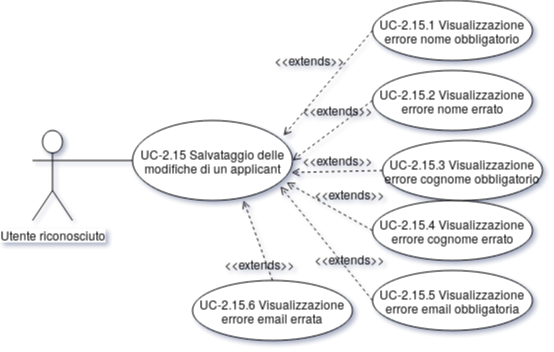
\includegraphics[width=1\columnwidth]{immagini/usecase/UC5} 
	\caption{Diagramma Use Case sulla visualizzazione errori relativi al salvataggio dell'applicant}
	\label{figura:uc-5}
\end{figure}


\paragraph{\underline{UC-2.15.1: Visualizzazione errore nome obbligatorio}}
\begin{itemize}	
	\item \textbf{Attori:} Utente riconosciuto
	\item \textbf{Precondizione:}  l'utente si trova nella vista di dettaglio di un applicant e ha tentato di cancellare del tutto il campo del nome di un applicant.
	\item \textbf{Scenario Principale:}
	\begin{enumerate}
		\item Viene visualizzato un errore che previene il salvataggio dei dati inconsistenti.
	\end{enumerate}
	\item \textbf{PostCondizione:} l'utente si trova nella vista di dettaglio di un applicant.
\end{itemize}

\paragraph{\underline{UC-2.15.2: Visualizzazione errore nome errato}}
\begin{itemize}	
	\item \textbf{Attori:} Utente riconosciuto
	\item \textbf{Precondizione:}  l'utente si trova nella vista di dettaglio di un applicant e ha tentato di inserire un nome con caratteri speciali.
	\item \textbf{Scenario Principale:}
	\begin{enumerate}
		\item Viene visualizzato un errore che previene il salvataggio dei dati inconsistenti.
	\end{enumerate}
	\item \textbf{PostCondizione:} l'utente si trova nella vista di dettaglio di un applicant.
\end{itemize}

\paragraph{\underline{UC-2.15.3: Visualizzazione errore cognome obbligatorio}}
\begin{itemize}	
	\item \textbf{Attori:} Utente riconosciuto
	\item \textbf{Precondizione:}  l'utente si trova nella vista di dettaglio di un applicant e ha tentato di cancellare del tutto il campo del cognome di un applicant.
	\item \textbf{Scenario Principale:}
	\begin{enumerate}
		\item Viene visualizzato un errore che previene il salvataggio dei dati inconsistenti.
	\end{enumerate}
	\item \textbf{PostCondizione:} l'utente si trova nella vista di dettaglio di un applicant.
\end{itemize}

\paragraph{\underline{UC-2.15.4: Visualizzazione errore cognome errato}}
\begin{itemize}	
	\item \textbf{Attori:} Utente riconosciuto
	\item \textbf{Precondizione:}  l'utente si trova nella vista di dettaglio di un applicant e ha tentato di inserire un cognome con caratteri speciali.
	\item \textbf{Scenario Principale:}
	\begin{enumerate}
		\item Viene visualizzato un errore che previene il salvataggio dei dati inconsistenti.
	\end{enumerate}
	\item \textbf{PostCondizione:} l'utente si trova nella vista di dettaglio di un applicant.
\end{itemize}

\paragraph{\underline{UC-2.15.5: Visualizzazione errore email obbligatoria}}
\begin{itemize}	
	\item \textbf{Attori:} Utente riconosciuto
	\item \textbf{Precondizione:}  l'utente si trova nella vista di dettaglio di un applicant e ha tentato di cancellare del tutto il campo della email di un applicant.
	\item \textbf{Scenario Principale:}
	\begin{enumerate}
		\item Viene visualizzato un errore che previene il salvataggio dei dati inconsistenti.
	\end{enumerate}
	\item \textbf{PostCondizione:} l'utente si trova nella vista di dettaglio di un applicant.
\end{itemize}

\paragraph{\underline{UC-2.15.6: Visualizzazione errore email errata}}
\begin{itemize}	
	\item \textbf{Attori:} Utente riconosciuto
	\item \textbf{Precondizione:}  l'utente si trova nella vista di dettaglio di un applicant e ha tentato di inserire una email che non rispetta il formato comunemente accettato.
	\item \textbf{Scenario Principale:}
	\begin{enumerate}
		\item Viene visualizzato un errore che previene il salvataggio dei dati inconsistenti.
	\end{enumerate}
	\item \textbf{PostCondizione:} l'utente si trova nella vista di dettaglio di un applicant.
\end{itemize}


\subsubsection{UC-2.16: Annullamento delle modifiche di un \applicant}
\begin{itemize}
	\item \textbf{Attori:} Utente riconosciuto
	\item \textbf{Precondizione:}  l'utente si trova nella vista di dettaglio di un applicant;
	\item \textbf{Scenario Principale:}
	\begin{enumerate}
		\item l'utente clicca sul pulsante di annullamento delle modifiche.
	\end{enumerate}
	\item \textbf{PostCondizione:} 
	\begin{enumerate}
		\item l'utente visualizza i campi dati nello stato antecedente alla modifica degli stessi;
		\item le modifiche vengono annullate;
		\item l'utente si trova nella vista di dettaglio di un applicant.
	\end{enumerate}
	
\end{itemize}


\subsubsection{\underline{UC-2.17: Modifica delle note generiche di un \applicant}}
\begin{itemize}
	\item \textbf{Attori:} Utente riconosciuto
	\item \textbf{Precondizione:}  l'utente si trova nella vista di dettaglio di un applicant;
	\item \textbf{Scenario Principale:}
	\begin{enumerate}
		\item l'utente clicca sul box di testo relativo alle note generiche;
		\item l'utente visualizza il  widget di inserimento testo relativo alle note generiche;
		\item l'utente inserisce le modifiche desiderate.
	\end{enumerate}
	\item \textbf{PostCondizione:} 
	\begin{enumerate}
		\item l'utente visualizza il campo dati modificato;
		\item l'utente si trova nella vista di dettaglio di un applicant.
	\end{enumerate}
	
\end{itemize}

\subsubsection{\underline{UC-2.18: Modifica delle note relative a un colloquio di un \applicant}}
\begin{itemize}
	\item \textbf{Attori:} Utente riconosciuto
	\item \textbf{Precondizione:}  l'utente si trova nella vista di dettaglio di un applicant;
	\item \textbf{Scenario Principale:}
	\begin{enumerate}
		\item l'utente clicca sul box di testo relativo alle note del colloquio;
		\item l'utente visualizza il  widget di inserimento testo relativo alle note del colloquio;
		\item l'utente inserisce le modifiche desiderate.
	\end{enumerate}
	\item \textbf{PostCondizione:} 
	\begin{enumerate}
		\item l'utente visualizza il campo dati modificato;
		\item l'utente si trova nella vista di dettaglio di un applicant.
	\end{enumerate}
	
\end{itemize}

\subsubsection{\underline{UC-2.19: Modifica delle note riguardanti lo status lavorativo di un \applicant}}
\begin{itemize}
	\item \textbf{Attori:} Utente riconosciuto
	\item \textbf{Precondizione:}  l'utente si trova nella vista di dettaglio di un applicant;
	\item \textbf{Scenario Principale:}
	\begin{enumerate}
		\item l'utente clicca sul box di testo relativo alle note generiche;
		\item l'utente visualizza il  widget di inserimento testo relativo alle note generiche;
		\item l'utente inserisce le modifiche desiderate.
	\end{enumerate}
	\item \textbf{PostCondizione:} 
	\begin{enumerate}
		\item l'utente visualizza il campo dati modificato;
		\item l'utente si trova nella vista di dettaglio di un applicant.
	\end{enumerate}
	
\end{itemize}

\subsubsection{\underline{UC-2.20: Modifica delle note riguardanti le considerazioni aggiuntive relative a un \applicant}}
\begin{itemize}
	\item \textbf{Attori:} Utente riconosciuto
	\item \textbf{Precondizione:}  l'utente si trova nella vista di dettaglio di un applicant;
	\item \textbf{Scenario Principale:}
	\begin{enumerate}
		\item l'utente clicca sul box di testo relativo alle note aggiuntive;
		\item l'utente visualizza il  widget di inserimento testo relativo alle note aggiuntive;
		\item l'utente inserisce le modifiche desiderate.
	\end{enumerate}
	\item \textbf{PostCondizione:} 
	\begin{enumerate}
		\item l'utente visualizza il campo dati modificato;
		\item l'utente si trova nella vista di dettaglio di un applicant.
	\end{enumerate}
	
\end{itemize}



\subsection{UC-3: Eliminazione di un\applicant}
\begin{itemize}
\item \textbf{Attori:}\loggedusr
\item \textbf{Precondizione:} l'utente si trova nella vista di visualizzazione lista degli applicant.
\item \textbf{Scenario Principale:}
\begin{enumerate}
	\item l'utente clicca il pulsante "Elimina" riferito a un certo applicant.
\end{enumerate}
\item \textbf{PostCondizione:} Viene visualizzato un messaggio di richiesta di conferma.
\end{itemize}

\subsubsection{\underline{UC-3.1: Conferma eliminazione di un\applicant}}
\begin{itemize}
	\item \textbf{Attori:}\loggedusr
	\item \textbf{Precondizione:}l'utente si trova nella vista di visualizzazione lista degli applicant e ha richiesto l'eliminazione di un applicant.
	\item \textbf{Scenario Principale:}
	\begin{enumerate}
		\item L'utente visualizza il messaggio di richiesta di conferma;
		\item L'utente preme il tasto "Ok".
	\end{enumerate}
	\item \textbf{PostCondizione:} si chiude il messaggio di conferma, avviene l'eliminazione dell'applicant e il \textit{refresh} della pagina.
	\item \textbf{Estensioni:} 
	\begin{enumerate}
		\item l'utente preme il tasto "Annulla";
		\item il messaggio di conferma viene chiuso.
	\end{enumerate}
\end{itemize}

\subsection{UC-4: Visualizzazione dettaglio di un \applicant }
\begin{itemize}
	\item \textbf{Attori:} \loggedusr
	\item \textbf{Precondizione:}  l'utente si trova nella vista di dettaglio di un applicant;
	\item \textbf{Scenario Principale:}
	\begin{enumerate}
		\item l'utente visualizza il nome dell'applicant (UC-4.1); 
		\item l'utente visualizza il cognome dell'applicant (UC-4.2);
		\item l'utente visualizza il genere dell'applicant (UC-4.3);
		\item l'utente visualizza la data di nascita dell'applicant (UC-4.4);
		\item l'utente visualizza l'email dell'applicant (UC-4.5);
		\item l'utente visualizza il numero di telefono dell'applicant (UC-4.6);	
		\item l'utente visualizza l'indirizzo dell'applicant (UC-4.7);
		\item l'utente visualizza la città residenza dell'applicant (UC-4.8);
		\item l'utente visualizza il preavviso richiesto dall'applicant per una chiamata (UC-4.9);
		\item l'utente visualizza il titolo di studio dell'applicant (UC-4.10);
		\item l'utente visualizza il livello di anzianità dell'applicant (UC-4.11);
		\item l'utente visualizza l'ambito di lavoro dell'applicant (UC-4.12);
		\item l'utente visualizza se lo status dell'applicant è scartato o meno (UC-4.13);
		\item l'utente visualizza le citta per cui l'applicant ha fornito disponibilità per il trasferimento (UC-4.14);
		\item l'utente visualizza delle note generiche relative all'applicant (UC-4.15);
		\item l'utente visualizza delle note relative al colloquio dell'applicant (UC-4.16);
		\item l'utente visualizza delle note riguardanti lo status lavorativo dell'applicant (UC-4.17);
		\item l'utente visualizza altre considerazioni aggiuntive relative all'applicant (UC-4.18).
	\end{enumerate}
	\item \textbf{PostCondizione:}  l'utente si trova nella vista di dettaglio di un applicant.
\end{itemize}

\begin{figure}[!h] 
	\centering 
	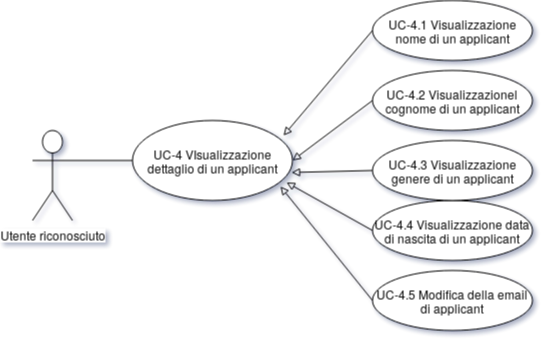
\includegraphics[width=1\columnwidth]{immagini/usecase/UC4} 
	\caption{Diagramma sottocasi UC-4}
	\label{figura:uc-4}
\end{figure}

\subsubsection{\underline{UC-4.1: Visualizzazione nome di un \applicant}}
\begin{itemize}
\item \textbf{Attori:} Utente riconosciuto
\item \textbf{Precondizione:} l'utente si trova nella vista di dettaglio di un applicant;
\item \textbf{Scenario Principale:}
\begin{enumerate} 
	\item l'utente visualizza il nome dell'applicant;
\end{enumerate}
\item \textbf{PostCondizione:} l'utente si trova nella vista di dettaglio di un applicant.
\end{itemize}

\subsubsection{\underline{UC-4.2: Visualizzazione cognome di un \applicant}}
\begin{itemize}
	\item \textbf{Attori:} Utente riconosciuto
	\item \textbf{Precondizione:} l'utente si trova nella vista di dettaglio di un applicant;
	\item \textbf{Scenario Principale:}
	\begin{enumerate} 
		\item l'utente visualizza il cognome dell'applicant;
	\end{enumerate}
	\item \textbf{PostCondizione:} l'utente si trova nella vista di dettaglio di un applicant.
\end{itemize}

\subsubsection{\underline{UC-4.3: Visualizzazione genere di un \applicant}}
\begin{itemize}
	\item \textbf{Attori:} Utente riconosciuto
	\item \textbf{Precondizione:} l'utente si trova nella vista di dettaglio di un applicant;
	\item \textbf{Scenario Principale:}
	\begin{enumerate} 
		\item l'utente visualizza il genere dell'applicant;
	\end{enumerate}
	\item \textbf{PostCondizione:} l'utente si trova nella vista di dettaglio di un applicant.
\end{itemize}

\subsubsection{\underline{UC-4.4: Visualizzazione data di nascita di un \applicant}}
\begin{itemize}
	\item \textbf{Attori:} Utente riconosciuto
	\item \textbf{Precondizione:} l'utente si trova nella vista di dettaglio di un applicant;
	\item \textbf{Scenario Principale:}
	\begin{enumerate} 
		\item l'utente visualizza il nome dell'applicant;
	\end{enumerate}
	\item \textbf{PostCondizione:} l'utente si trova nella vista di dettaglio di un applicant.
\end{itemize}

\subsubsection{\underline{UC-4.5: Visualizzazione email di un \applicant}}
\begin{itemize}
	\item \textbf{Attori:} Utente riconosciuto
	\item \textbf{Precondizione:} l'utente si trova nella vista di dettaglio di un applicant;
	\item \textbf{Scenario Principale:}
	\begin{enumerate} 
		\item l'utente visualizza il nome dell'applicant;
	\end{enumerate}
	\item \textbf{PostCondizione:} l'utente si trova nella vista di dettaglio di un applicant.
\end{itemize}

\subsubsection{\underline{UC-4.6: Visualizzazione numero di telefono di un \applicant}}
\begin{itemize}
	\item \textbf{Attori:} Utente riconosciuto
	\item \textbf{Precondizione:} l'utente si trova nella vista di dettaglio di un applicant;
	\item \textbf{Scenario Principale:}
	\begin{enumerate} 
		\item l'utente visualizza il numero di telefono dell'applicant;
	\end{enumerate}
	\item \textbf{PostCondizione:} l'utente si trova nella vista di dettaglio di un applicant.
\end{itemize}

\subsubsection{\underline{UC-4.7: Visualizzazione l'indirizzo di un \applicant}}
\begin{itemize}
	\item \textbf{Attori:} Utente riconosciuto
	\item \textbf{Precondizione:} l'utente si trova nella vista di dettaglio di un applicant;
	\item \textbf{Scenario Principale:}
	\begin{enumerate} 
		\item l'utente visualizza l'indirizzo dell'applicant;
	\end{enumerate}
	\item \textbf{PostCondizione:} l'utente si trova nella vista di dettaglio di un applicant.
\end{itemize}

\subsubsection{\underline{UC-4.8: Visualizzazione città di residenza di un \applicant}}
\begin{itemize}
	\item \textbf{Attori:} Utente riconosciuto
	\item \textbf{Precondizione:} l'utente si trova nella vista di dettaglio di un applicant;
	\item \textbf{Scenario Principale:}
	\begin{enumerate} 
		\item l'utente visualizza la città di residenza dell'applicant;
	\end{enumerate}
	\item \textbf{PostCondizione:} l'utente si trova nella vista di dettaglio di un applicant.
\end{itemize}

\subsubsection{\underline{UC-4.9: Visualizzazione preavviso richiesto da un \applicant}}
\begin{itemize}
	\item \textbf{Attori:} Utente riconosciuto
	\item \textbf{Precondizione:} l'utente si trova nella vista di dettaglio di un applicant;
	\item \textbf{Scenario Principale:}
	\begin{enumerate} 
		\item l'utente visualizza il preavviso richiesto dall'applicant;
	\end{enumerate}
	\item \textbf{PostCondizione:} l'utente si trova nella vista di dettaglio di un applicant.
\end{itemize}

\subsubsection{\underline{UC-4.10: Visualizzazione titolo di studio di un \applicant}}
\begin{itemize}
	\item \textbf{Attori:} Utente riconosciuto
	\item \textbf{Precondizione:} l'utente si trova nella vista di dettaglio di un applicant;
	\item \textbf{Scenario Principale:}
	\begin{enumerate} 
		\item l'utente visualizza il titolo di studio dell'applicant;
	\end{enumerate}
	\item \textbf{PostCondizione:} l'utente si trova nella vista di dettaglio di un applicant.
\end{itemize}

\subsubsection{\underline{UC-4.11: Visualizzazione livello di anzianità di un \applicant}}
\begin{itemize}
	\item \textbf{Attori:} Utente riconosciuto
	\item \textbf{Precondizione:} l'utente si trova nella vista di dettaglio di un applicant;
	\item \textbf{Scenario Principale:}
	\begin{enumerate} 
		\item l'utente visualizza il livello di anzianità dell'applicant;
	\end{enumerate}
	\item \textbf{PostCondizione:} l'utente si trova nella vista di dettaglio di un applicant.
\end{itemize}

\subsubsection{\underline{UC-4.12: Visualizzazione ambito lavorativo di un \applicant}}
\begin{itemize}
	\item \textbf{Attori:} Utente riconosciuto
	\item \textbf{Precondizione:} l'utente si trova nella vista di dettaglio di un applicant;
	\item \textbf{Scenario Principale:}
	\begin{enumerate} 
		\item l'utente visualizza l'ambito lavorativo dell'applicant;
	\end{enumerate}
	\item \textbf{PostCondizione:} l'utente si trova nella vista di dettaglio di un applicant.
\end{itemize}

\subsubsection{\underline{UC-4.13: Visualizzazione status (scartato o meno) di un \applicant}}
\begin{itemize}
	\item \textbf{Attori:} Utente riconosciuto
	\item \textbf{Precondizione:} l'utente si trova nella vista di dettaglio di un applicant;
	\item \textbf{Scenario Principale:}
	\begin{enumerate} 
		\item l'utente visualizza se lo status dell'applicant è scartato o meno;
	\end{enumerate}
	\item \textbf{PostCondizione:} l'utente si trova nella vista di dettaglio di un applicant.
\end{itemize}

\subsubsection{\underline{UC-4.14: Visualizzazione disponibilità geografica di un \applicant}}
\begin{itemize}
	\item \textbf{Attori:} Utente riconosciuto
	\item \textbf{Precondizione:} l'utente si trova nella vista di dettaglio di un applicant;
	\item \textbf{Scenario Principale:}
	\begin{enumerate} 
		\item l'utente visualizza le città per cui l'applicant ha fornito disponibilità per il trasferimento;
	\end{enumerate}
	\item \textbf{PostCondizione:} l'utente si trova nella vista di dettaglio di un applicant.
\end{itemize}

\subsubsection{\underline{UC-4.15: Visualizzazione note generiche di un \applicant}}
\begin{itemize}
	\item \textbf{Attori:} Utente riconosciuto
	\item \textbf{Precondizione:} l'utente si trova nella vista di dettaglio di un applicant;
	\item \textbf{Scenario Principale:}
	\begin{enumerate} 
		\item l'utente visualizza le note generiche relative all'applicant;
	\end{enumerate}
	\item \textbf{PostCondizione:} l'utente si trova nella vista di dettaglio di un applicant.
\end{itemize}

\subsubsection{\underline{UC-4.16: Visualizzazione note relative al colloquio di un \applicant}}
\begin{itemize}
	\item \textbf{Attori:} Utente riconosciuto
	\item \textbf{Precondizione:} l'utente si trova nella vista di dettaglio di un applicant;
	\item \textbf{Scenario Principale:}
	\begin{enumerate} 
		\item l'utente visualizza le note relative al colloquio dell'applicant;
	\end{enumerate}
	\item \textbf{PostCondizione:} l'utente si trova nella vista di dettaglio di un applicant.
\end{itemize}


\subsubsection{\underline{UC-4.17: Visualizzazione note sullo status lavorativo di un \applicant}}
\begin{itemize}
	\item \textbf{Attori:} Utente riconosciuto
	\item \textbf{Precondizione:} l'utente si trova nella vista di dettaglio di un applicant;
	\item \textbf{Scenario Principale:}
	\begin{enumerate} 
		\item l'utente visualizza note riguardanti lo status lavorativo dell'applicant;
	\end{enumerate}
	\item \textbf{PostCondizione:} l'utente si trova nella vista di dettaglio di un applicant.
\end{itemize}


\subsubsection{\underline{UC-4.18: Visualizzazione note aggiuntive relative a un \applicant}}
\begin{itemize}
	\item \textbf{Attori:} Utente riconosciuto
	\item \textbf{Precondizione:} l'utente si trova nella vista di dettaglio di un applicant;
	\item \textbf{Scenario Principale:}
	\begin{enumerate} 
		\item l'utente visualizza note riguardanti le considerazioni aggiunitve relative all'applicant;
	\end{enumerate}
	\item \textbf{PostCondizione:} l'utente si trova nella vista di dettaglio di un applicant.
\end{itemize}

\vspace{0.5em}
\begin{figure}[!h]
	\centering 
	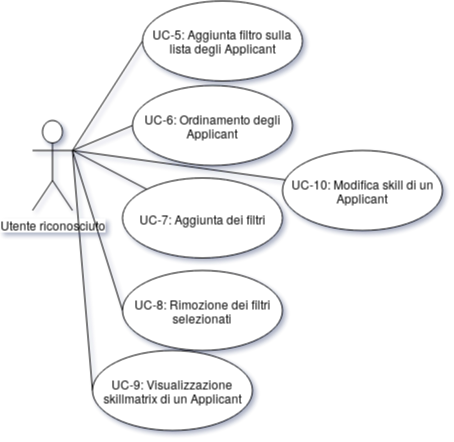
\includegraphics[width=0.7\columnwidth]{immagini/usecase/UC6} 
	\caption{Diagramma di Use Case da UC-5 a UC-10}
	\label{figura:uc-6}
\end{figure}

\subsection{UC-5: Aggiunta filtro sulla lista degli\applicant}
\begin{itemize}
	\item \textbf{Attori:}\loggedusr
	\item \textbf{Precondizione:} l'utente si trova nella vista di visualizzazione lista degli applicant.
	\item \textbf{Scenario Principale:}
	\begin{enumerate}
		\item l'utente inserisce nel campo di testo un carattere o un insieme di caratteri.
	\end{enumerate}
	\item \textbf{PostCondizione:} viene visualizzata la lista degli applicant dove nome e cognome contengono i caratteri inseriti.
\end{itemize}


\vspace{0.5em}
\begin{figure}[!h] UC-7.1 Visualizzazione errore sulla selezione dei filtri
	\centering 
	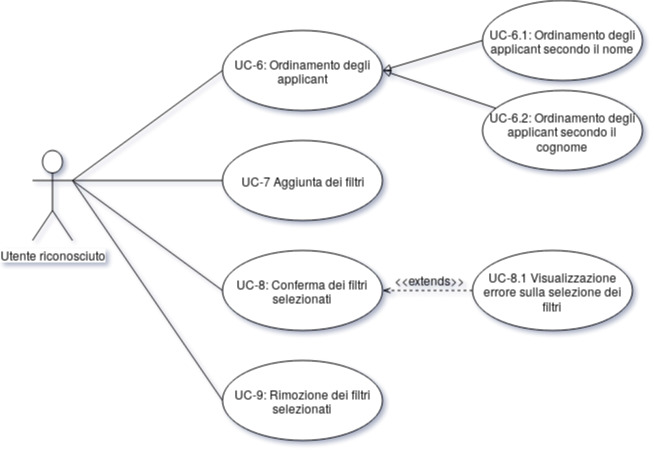
\includegraphics[width=1\columnwidth]{immagini/usecase/UC2} 
	\caption{Diagramma di Use Case delle operazioni ausiliare sulla lista degli applicant}
	\label{figura:uc-2}
\end{figure}

\subsection{UC-6: Ordinamento degli\applicant}
\begin{itemize}
	\item \textbf{Attori:}\loggedusr
	\item \textbf{Precondizione:} l'utente si trova nella vista di visualizzazione lista degli applicant.
	\item \textbf{Scenario Principale:}
	\begin{enumerate}
		\item l'utente clicca sul \textit{header} della lista riportante il campo desiderato;
		\item gli applicant vengono posti in ordine crescente secondo il campo desiderato.
	\end{enumerate}
	\item \textbf{PostCondizione:}  l'utente si trova nella vista di visualizzazione lista degli applicant.
\end{itemize}


\subsubsection{\underline{UC-6.1: Ordinamento degli\applicant secondo il nome}}
\begin{itemize}
	\item \textbf{Attori:}\loggedusr
	\item \textbf{Precondizione:} l'utente si trova nella vista di visualizzazione lista degli applicant.
	\item \textbf{Scenario Principale:}
	\begin{enumerate}
		\item l'utente clicca sul \textit{header} della lista riportante il campo "Nome";
		\item gli applicant vengono posti in ordine crescente secondo il nome.
	\end{enumerate}
	\item \textbf{PostCondizione:}  l'utente si trova nella vista di visualizzazione lista degli applicant.
\end{itemize}

\subsubsection{\underline{UC-6.2: Ordinamento degli\applicant secondo il cognome}}
\begin{itemize}
	\item \textbf{Attori:}\loggedusr
	\item \textbf{Precondizione:} l'utente si trova nella vista di visualizzazione lista degli applicant.
	\item \textbf{Scenario Principale:}
	\begin{enumerate}
		\item l'utente clicca sul \textit{header} della lista riportante il campo "Cognome";
		\item gli applicant vengono posti in ordine crescente secondo il cognome.
	\end{enumerate}
	\item \textbf{PostCondizione:}  l'utente si trova nella vista di visualizzazione lista degli applicant.
\end{itemize}

\subsection{UC-7: Aggiunta dei filtri}
\begin{itemize}
\item \textbf{Attori:}\loggedusr
\item \textbf{Precondizione:} l'utente si trova nella vista relativa ai filtri.
\item \textbf{Scenario Principale:}
\begin{enumerate}
	\item l'utente aggiunge un filtro mediante l'inserimento di un input;
\end{enumerate}
\item \textbf{PostCondizione:} l'utentesi trova nella vista relativa ai filtri e visualizza l'input immesso sullo schermo.
\end{itemize}

\subsubsection{\underline{UC7.1: Aggiunta di un filtro per il nome}}
\begin{itemize}
\item \textbf{Attori:}\loggedusr
\item \textbf{Precondizione:} l'utente si trova nella vista relativa ai filtri.
\item \textbf{Scenario Principale:}
\begin{enumerate}
	\item l'utente inserisce una parola chiave in un campo di testo dedicato al nome;
\end{enumerate}
\item \textbf{PostCondizione:}  l'utente si trova nella vista relativa ai filtri e visualizza l'input immesso sullo schermo.
\end{itemize}

\subsubsection{\underline{UC7.2: Aggiunta di un filtro per il cognome}}
\begin{itemize}
	\item \textbf{Attori:}\loggedusr
	\item \textbf{Precondizione:} l'utente si trova nella vista relativa ai filtri.
	\item \textbf{Scenario Principale:}
	\begin{enumerate}
		\item l'utente inserisce una parola chiave in un campo di testo dedicato al cognome.
	\end{enumerate}
	\item \textbf{PostCondizione:}  l'utente si trova nella vista relativa ai filtri e visualizza l'input immesso sullo schermo.
\end{itemize}

\subsubsection{\underline{UC-7.3: Aggiunta di un filtro per il genere}}
\begin{itemize}
	\item \textbf{Attori:}\loggedusr
	\item \textbf{Precondizione:} l'utente si trova nella vista relativa ai filtri.
	\item \textbf{Scenario Principale:}
	\begin{enumerate}
		\item l'utente seleziona da un menù a tendina il genere desiderato.
	\end{enumerate}
	\item \textbf{PostCondizione:}  l'utente si trova nella vista relativa ai filtri e visualizza l'opzione selezionata sullo schermo.
\end{itemize}

\subsubsection{\underline{UC-7.4: Aggiunta di un filtro per il titolo di studio}}
\begin{itemize}
	\item \textbf{Attori:}\loggedusr
	\item \textbf{Precondizione:} l'utente si trova nella vista relativa ai filtri.
	\item \textbf{Scenario Principale:}
	\begin{enumerate}
		\item l'utente seleziona da un menù a tendina il titolo di studio desiderato.
	\end{enumerate}
	\item \textbf{PostCondizione:}  l'utente si trova nella vista relativa ai filtri e visualizza l'opzione selezionata sullo schermo.
\end{itemize}
\subsubsection{\underline{UC-7.5: Aggiunta di un filtro per l'ambito lavorativo}}
\begin{itemize}
	\item \textbf{Attori:}\loggedusr
	\item \textbf{Precondizione:} l'utente si trova nella vista relativa ai filtri.
	\item \textbf{Scenario Principale:}
	\begin{enumerate}
		\item l'utente seleziona da un menù a tendina l'ambito lavorativo desiderato.
	\end{enumerate}
	\item \textbf{PostCondizione:}  l'utente si trova nella vista relativa ai filtri e visualizza l'opzione selezionata sullo schermo.
\end{itemize}

\subsubsection{\underline{UC-7.6: Aggiunta di un filtro relativo ad una skill }}
\begin{itemize}
	\item \textbf{Attori:}\loggedusr
	\item \textbf{Precondizione:} l'utente si trova nella vista relativa ai filtri.
	\item \textbf{Scenario Principale:}
	\begin{enumerate}
		\item l'utente seleziona da un menù a tendina il nome della skill desiderato.
	\end{enumerate}
	\item \textbf{PostCondizione:}  l'utente si trova nella vista relativa ai filtri e visualizza l'opzione selezionata sullo schermo.
\end{itemize}

\subsubsection{\underline{UC-7.7: Aggiunta di un filtro relativo al livello di una skill}}
\begin{itemize}
	\item \textbf{Attori:}\loggedusr
	\item \textbf{Precondizione:} l'utente si trova nella vista relativa ai filtri.
	\item \textbf{Scenario Principale:}
	\begin{enumerate}
		\item l'utente seleziona da un menù a tendina un valore da 1 a 4 rappresentante il livello della skill desiderato.
	\end{enumerate}
	\item \textbf{PostCondizione:}  l'utente si trova nella vista relativa ai filtri e visualizza l'opzione selezionata sullo schermo.
\end{itemize}


\subsubsection{\underline{UC-7.8: Aggiunta di un filtro per la disponibilità geografica}}
\begin{itemize}
	\item \textbf{Attori:}\loggedusr
	\item \textbf{Precondizione:} l'utente si trova nella vista relativa ai filtri.
	\item \textbf{Scenario Principale:}
	\begin{enumerate}
		\item l'utente seleziona una o più città desiderate.
	\end{enumerate}
	\item \textbf{PostCondizione:}  l'utente si trova nella vista relativa ai filtri e visualizza le opzioni selezionate sullo schermo.
\end{itemize}

\subsubsection{\underline{UC-7.9: Aggiunta di un filtro per l'anzianità}}
\begin{itemize}
	\item \textbf{Attori:}\loggedusr
	\item \textbf{Precondizione:} l'utente si trova nella vista relativa ai filtri.
	\item \textbf{Scenario Principale:}
	\begin{enumerate}
		\item l'utente seleziona da un menù a tendina il livello di anzianità desiderato.
	\end{enumerate}
	\item \textbf{PostCondizione:}  l'utente si trova nella vista relativa ai filtri e visualizza l'opzione selezionata sullo schermo.
\end{itemize}

\subsubsection{\underline{UC-7.10: Conferma dei filtri selezionati}}
\begin{itemize}
\item \textbf{Attori:}\loggedusr
\item \textbf{Precondizione:} l'utente si trova nella vista relativa ai filtri.
\item \textbf{Scenario Principale:}
\begin{enumerate}
	\item l'utente clicca sul tasto "Applica filtri selezionati";
	\item l'utente viene reindirizzato alla vista di visualizzazione lista degli applicant.
\end{enumerate}
\item \textbf{PostCondizione:} l'utente si trova nella vista relativa alla visualizzazione degli applicant e visualizza li visualizza secondo i filtri selezionati;
\item \textbf{Estensioni:} l'utente visualizza un messaggio di errore relativo all'inserimento dei filtri (UC-7.11.1);
\end{itemize}

\paragraph{\underline{UC-7.10.1: Visualizzazione errore sulla selezione dei filtri}}
\begin{itemize}
\item \textbf{Attori:}\loggedusr
\item \textbf{Precondizione:} l'utente si trova nella vista relativa ai filtri e non ha selezionato congiuntamente una skill e un livello, ma solo uno dei due.
\item \textbf{Scenario Principale:}
\begin{enumerate}
	\item viene visualizzato un errore a schermo che invita l'utente a completare la selezione dei filtri.
\end{enumerate}
\item \textbf{PostCondizione:}l'utente si trova nella vista relativa ai filtri.
\end{itemize}


\subsection{UC-8: Rimozione dei filtri selezionati}
\begin{itemize}
\item \textbf{Attori:}\loggedusr
\item \textbf{Precondizione:} l'utente si trova nella vista relativa ai filtri
\item \textbf{Scenario Principale:}
\begin{enumerate}
	\item l'utente clicca sul tasto "Annulla";
	\item vengono rimossi tutti i flitri precedentemente selezionati.
\end{enumerate}
\item \textbf{PostCondizione:} l'utente si trova nella vista relativa ai filtri.
\end{itemize}

\subsection{UC-9: Visualizzazione skillmatrix di un \applicant}
\begin{itemize}
\item \textbf{Attori:} Utente riconosciuto
\item \textbf{Precondizione:}  l'utente si trova nella vista di dettaglio di un applicant
\item \textbf{Scenario Principale:}
\begin{enumerate}
	\item l'utente clicca sul pulsante relativo alla visualizzazione skillmatrix di un applicant
\end{enumerate}
\item \textbf{PostCondizione:} l'utente si trova nella vista relativa alla visualizzazione skillmatrix di un applicant.
\end{itemize}

\subsubsection{UC-9.1: Visualizzazione nome della skill}
\begin{itemize}
\item \textbf{Attori:} Utente riconosciuto
\item \textbf{Precondizione:}  l'utente si trova nella vista relativa alla visualizzazione skillmatrix di un applicant.
\item \textbf{Scenario Principale:}
\begin{enumerate}
	\item l'utente visualizza il nome della skill posseduta dall'applicant
\end{enumerate}
\item \textbf{PostCondizione:}  l'utente si trova nella vista relativa alla visualizzazione skillmatrix di un applicant.
\end{itemize}

\subsubsection{UC-9.2: Visualizzazione livello della skill}
\begin{itemize}
	\item \textbf{Attori:} Utente riconosciuto
	\item \textbf{Precondizione:}  l'utente si trova nella vista relativa alla visualizzazione skillmatrix di un applicant.
	\item \textbf{Scenario Principale:}
	\begin{enumerate}
		\item l'utente visualizza il livello della skill posseduta dall'applicant
	\end{enumerate}
	\item \textbf{PostCondizione:}  l'utente si trova nella vista relativa alla visualizzazione skillmatrix di un applicant.
\end{itemize}



\subsection{UC-10: Modifica skill di un \applicant}
\begin{itemize}
\item \textbf{Attori:} Utente riconosciuto
\item \textbf{Precondizione:} l'utente si trova nella vista relativa alla visualizzazione skillmatrix di un applicant.
\item \textbf{Scenario Principale:}
\begin{enumerate}
	\item l'utente seleziona una skill da modificare;
	\item l'utente seleziona il livello desiderato da un menù a tendina.
\end{enumerate}
\item \textbf{PostCondizione:} l'utente si trova nella vista relativa alla visualizzazione skillmatrix di un applicant e viene visualizzato un pulsante di conferma.
\end{itemize}

\subsubsection{\underline{UC-10.1: Conferma della modifica skill di un \applicant}}
\begin{itemize}
	\item \textbf{Attori:} Utente riconosciuto
	\item \textbf{Precondizione:} l'utente si trova nella vista relativa alla visualizzazione skillmatrix di un applicant e ha effettuato una modifica su uno o più livelli di una skill.
	\item \textbf{Scenario Principale:}
	\begin{enumerate}
		\item l'utente clicca sul pulsante di conferma.
	\end{enumerate}
	\item \textbf{PostCondizione:} l'utente si trova nella vista relativa alla visualizzazione skillmatrix di un applicant e le modifiche precedentemente apportate risultano salvate.
\end{itemize}

\subsubsection{\underline{UC-10.2: Annullamento della modifica skill di un\applicant}}
\begin{itemize}
	\item \textbf{Attori:} Utente riconosciuto
	\item \textbf{Precondizione:} l'utente si trova nella vista relativa alla visualizzazione skillmatrix di un applicant e ha effettuato una modifica su uno o più livelli di una skill.
	\item \textbf{Scenario Principale:}
	\begin{enumerate}
		\item l'utente clicca sul pulsante di annullamento.
	\end{enumerate}
	\item \textbf{PostCondizione:} l'utente si trova nella vista relativa alla visualizzazione skillmatrix di un applicant e le modifiche precedentemente apportate vengono eliminate, ripristinando lo stato originale dello skillmatrix.
\end{itemize}

\section{Tracciamento dei requisiti}
In corrispondenza dell'analisi degli use case effettuata effettuata con il supporto del tutor aziendale, vengono identificati i requisiti relativi al progetto di stage, essi sono definiti secondo la seguente notazione:
\vspace{1em}
\begin{center}
	R(Importanza)(Tipologia)(Codice)
\end{center}

Dove per ciascun parametro possono essere assegnate le seguenti opzioni:
\begin{itemize}
	\item Importanza
	\begin{itemize}
		\item O: indica un requisito obbligatorio
		\item D: indica un requisito desiderabile
		\item P: indica un requisito facoltativo (opzionale)
	\end{itemize}
	\item Tipologia
	\begin{itemize}
		\item F : indica un requisito funzionale. Rappresenta le funzionalità che il prodotto
		deve fornire.
		\item Q : indica un requisito qualitativo. Rappresenta gli elementi per aumentare
		la qualità del prodotto finale
		\item  P : indica un requisito prestazionale. Rappresenta un valore misurabile delle
		performance raggiunte dal prodotto terminato.
		\item V : indica un requisito di vincolo. Rappresenta le limitazioni che il prodotto
		deve rispettare.
	\end{itemize}
	\item Codice : un codice progressivo utile per identificare univocamente i requisiti individuati.
\end{itemize}

\subsection{Requisiti funzionali}
\begin{center}
	\begin{tabularx}{\textwidth}{|c|X|c|}
		\hline
		\textbf{Codice} & \textbf{Descrizione} & \textbf{Use Case} \\
		\hline
		\endhead
		ROF01 & L'utente riconosciuto deve poter visualizzare la lista degli applicant registrati presso SyncRec & UC-1 \\
		\hline
		ROF02 & L'utente deve poter accedere alla vista di dettaglio di un applicant a partire dalla lista del totale delle persone richiedenti registrate & UC-1.1 \\
		\hline
		ROF03 & L'utente deve poter modificare i dati registrati di un applicant & UC-2 \\
		\hline
		ROF04 & L'utente deve poter modificare il nome di un applicant & UC-2.1 \\
		\hline
		ROF05 & L'utente deve poter modificare il nome di un applicant & UC-2.2 \\
		\hline
		ROF06 & L'utente deve poter modificare il genere di un applicant & UC-2.3\\
		\hline
		ROF07 & L'utente deve poter modificare l'indirizzo di un applicant & UC-2.4 \\
		\hline
		ROF08 &  L'utente deve poter modificare la data di nascita di un applicant & UC-2.5 \\
		\hline
		ROF09 & L'utente deve poter modificare la città di residenza di un applicant & UC 2.6 \\
		\hline
		ROF10 & L'utente deve poter modificare l'email di un applicant & UC-2.7\\
		\hline
		ROF11 & L'utente deve poter modificare l'ambito lavorativo di un applicant &  UC-2.8\\
		\hline
		ROF12 & L'utente deve poter modificare il titolo di studio di un applicant & UC-2.10 \\
		\hline
		ROF13 & L'utente deve poter modificare la disponibilità geografica di un applicant & UC-2.11\\
		\hline
		ROF14 & L'utente deve poter modificare il tempo di preavviso di un applicant & UC-2.12\\
		\hline
		ROF15 & L'utente deve poter modificare il telefono di un applicant & UC-2.13 \\
		\hline
		ROF16 & L'utente deve poter scaricare il curriculum di un applicant & UC-2.14\\
		\hline
		ROF17 & L'utente deve poter confermare le modifiche apportate a un applicant & UC-2.15 \\
		\hline
		ROF18 & L'utente deve poter annullare le modifiche apportate a un applicant &  UC-2.16\\
		\hline
		ROF19 & L'utente deve poter visualizzare un messaggio di errore se il nome non è presente & UC-2.15.1 \\
		\hline
		ROF20 & L'utente deve poter visualizzare un messaggio di errore se il nome presenta dei caratteri non alfabetici & 2.15.2 \\
		\hline
		ROF21 & L'utente deve poter visualizzare un messaggio di errore se il cognome non è presente & UC-2.15.3 \\
		\hline
		ROF22 & L'utente deve poter visualizzare un messaggio di errore se il cognome presenta dei caratteri non alfabetici & UC-2.15.4\\
		\hline
		ROF23 & L'utente deve poter visualizzare un messaggio di errore se l'email non è presente & UC-2.15.5\\
		\hline
		ROF24 & L'utente deve poter visualizzare un messaggio di errore se l'email presenta una struttura non corretta & UC-2.15.6\\
		\hline
		ROF24 & L'utente deve poter modificare le note generiche di un applicant & UC-2.17 \\
		\hline
		ROF25 & L'utente deve poter modificare le note relative al colloquio di un applicant & UC-2.18 \\
		\hline
		ROF26 & L'utente deve poter le note riguardanti lo status lavorativo di un applicant & UC-2.19\\
		\hline
		ROF27 & L'utente deve poter mopdificare le note riguardanti le considerazioni aggiuntive relative a un applicant &  UC-2.20\\
		\hline
		ROF28 & L'utente deve poter eliminare definitivamente un applicant & UC-3 \\
		\hline
		ROF29 & L'utente deve poter confermare l'eliminazione di un applicant & UC-3.1 \\
		\hline
		ROF30 & L'utente deve poter visualizzare il dettaglio di un applicant & UC-4 \\
		\hline
		ROF31 & L'utente deve poter visualizzare il nome di un applicant & UC-4.1\\
		\hline
		ROF32 & L'utente deve poter visualizzare il cognome di un applicant  & UC-4.2 \\
		\hline
		ROF33 & L'utente deve poter visualizzare il genere di un applicant & UC-4.3\\
		\hline
		ROF34 & L'utente deve poter visualizzare la data di nascita di un applicant& UC-4.4 \\
		\hline
		ROF35 & L'utente deve poter visualizzare l'email di un applicant& UC-4.5\\
		\hline
		ROF36 & L'utente deve poter visualizzare il numero di telefono di un applicant& UC-4.6\\
		\hline
		ROF37 & L'utente deve poter visualizzare l'indirizzo di un applicant& UC-4.7\\
		\hline
		ROF38 & L'utente deve poter visualizzare la città di residenza di un applicant&  UC-4.8\\
		\hline
		ROF39 & L'utente deve poter visualizzare il preavviso richiesto da un applicant & UC-4.9 \\
		\hline
		ROF40 &  L'utente deve poter visualizzare il titolo di studio di un applicant & UC-4.10\\
		\hline 
		ROF41 &  L'utente deve poter visualizzare il livello di anzianità di un applicant& UC-4.11\\
		\hline
		ROF42 &  L'utente deve poter visualizzare l'ambito di lavoro di un applicant& UC-4.12\\
		\hline
		ROF43 &  L'utente deve poter visualizzare se l'applicant è scartato o meno & UC-4.13\\
		\hline
		ROF44 &  L'utente deve poter visualizzare le note generiche relative a un applicant & UC-4.15\\
		\hline
		ROF45 &  L'utente deve poter visualizzare le note relative al colloquio dell'applicant & UC-4.16\\
		\hline
		ROF46 &  L'utente deve poter visualizzare le note relative allo status lavorativo dell'applicant& UC-4.17\\
		\hline
		ROF47 & L'utente deve poter visualizzare altre considerazioni aggiuntive relative all'applicant & UC-4.18\\
		\hline
		ROF48 & L'utente deve poter filtrare la lista degli applicant secondo il nome e cognome & UC-5\\
		\hline
		ROF49 & L'utente deve poter ordinare la lista degli applicant secondo determinati criteri & UC-6 \\
		\hline
		ROF50 & L'utente deve poter ordinare la lista degli applicant secondo il nome & UC-6.1\\
		\hline
		ROF51 & L'utente deve poter ordinare la lista degli applicant secondo il cognome & UC-6.2\\
		\hline
		ROF52 & L'utente deve poter aggiungere filtri alla lista degli applicant secondo determinati criteri &  UC-7\\
		\hline
		ROF53 & L'utente deve aggiungere un filtro per il nome sulla lista degli applicant & UC-7.1 \\
		\hline
		ROF54 & L'utente deve aggiungere un filtro per il cognome sulla lista degli applicant & UC-7.2\\
		\hline
		ROF55 & L'utente deve aggiungere un filtro per il genere sulla lista degli applicant & UC-7.3\\
		\hline
		ROF56 & L'utente deve aggiungere un filtro per il titolo di studio sulla lista degli applicant & UC-7.4 \\
		\hline
		ROF57 & L'utente deve aggiungere un filtro per l'ambito lavorativo sulla lista degli applicant & UC-7.5\\
		\hline
		ROF58 & L'utente deve aggiungere un filtro per il nome di una skill sulla lista degli applicant &  UC-7.6 \\
		\hline
		ROF59 & L'utente deve aggiungere un filtro per il livello di una skill sulla lista degli applicant & UC-7.7 \\
		\hline
		ROF60 & L'utente deve aggiungere un filtro per la disponibilità geografica di un applicant& UC-7.8\\
		\hline
		ROF61 & L'utente deve aggiungere un filtro per l'anzianità di un applicant& UC-7.9\\
		\hline
		ROF62 & L'utente deve poter confermare l'aggiunta dei filtri selezionati& UC-7.10\\
		\hline
		ROF63 & L'utente deve poter annullare l'aggiunta dei filtri selezionati& UC-7.11\\
		\hline
		ROF64 & L'utente deve poter visualizzare un eventuale errore commesso nell'aggiunta dei filtri & 7.10.1 \\
		\hline
		ROF65 & L'utente deve poter rimuovere i filtri precedentemente selezionati & UC-8\\
		\hline
		ROF66 & L'utente deve poter visualizzare lo skillmatrix di un applicant & UC-9\\
		\hline
		ROF67 & L'utente deve poter visualizzare il nome di una skill posseduta da un applicant & UC-9.1 \\
		\hline
		ROF68 & L'utente deve poter visualizzare il livello di una skill posseduta da un applicant & UC-9.2\\
		\hline
		ROF69 &L'utente deve poter modificare il livello di una skill posseduta da un applicant &  UC-10\\
		\hline
		ROF70 &  L'utente deve poter confermare le modifiche apportate allo skillmatrix di un applicant& UC-10.1\\
		\hline
		ROF71 & L'utente deve poter annullare le modifiche apportate allo skillmatrix di un applicant & UC-10.2 \\
		\hline
	\end{tabularx}
\end{center}


\subsection{Requisiti di vincolo}
\begin{center}
	\begin{tabularx}{\textwidth}{|c|X|}
		\hline
		\textbf{Codice} & \textbf{Descrizione} \\
		\hline
		ROV01 & Utilizzo del framework Angular per lo sviluppo dell'applicazione\\
		\hline
		ROV02 & Utilizzo di MongoDb per la gestione dei dati\\
		\hline
		ROV03 & Utilizzo di Spring per il back-end
		dell'applicazione\\
		\hline
		ROV04 & Utilizzo di Visual Studio Code come \gls{IDE}\\
		\hline
	\end{tabularx}
\end{center}



